\chapter{Heat Transfer}\label{ch_Heat_Transfer}
Inside trapezoidal cavity receiver heat transfer takes place via convection (conduction and advection) and radiation. Since air is present inside trapezoidal cavity receiver, it will lead to convection given temperature difference. Apart from that Top, left and right walls of the cavity, bottom glass cover and pipes will be exchanging heat via radiation. Temperature gradient inside the trapezoidal cavity receiver will lead to convection. However, the possibility of convection depends on the relative direction of the temperature gradient with respect to the gravity.  Consider two vectors, first representing the direction of temperature gradient and second representing the direction of gravity. When the first vector is in the direction of the second vector, the maximum amount of convection takes place as due to density difference hot water will float and it will have a tendency of moving opposite of the direction of gravity while colder air will have a tendency to move in the direction of gravity. This phenomenon will continue until temperature gradient vector is completely opposite of the gravity, which is the scenario in our study. Experiments done on the trapezoidal cavity receiver shows that top wall of the cavity is at a higher temperature relative to the bottom glass temperature. In this case, temperature gradient vector is opposite to the gravity so, convection should not occur. However, since there are other parts like pipes through which working fluid is passing through temperature gradient exists in the lateral direction as well. But experiments and simulations performed on trapezoidal cavity receiver show that these temperature gradients are quite smaller than the temperature gradient existing between the top wall and the bottom glass. Thus even though some local convective currents do form. Its contribution to the overall heat transfer is very low. Mohan et. al.\citep{MOHAN201837} have shown that contribution of advection in convection inside trapezoidal cavity receiver is very low. To show that two simulations were performed by him. Inside trapezoidal cavity receiver, heat transfer was modeled with convection (conduction and advection) in one case while in another case it was modeled with conduction alone. The result shows less than 1 \% of a difference in the Nusselt number at the hot wall obtained in both the simulations. Keeping that in mind, in the present work heat transfer has been modeled with conduction only and advection has been ignored. To verify the conduction model same problem is solved here as has been by Mohan et. al.\citep{MOHAN201837} and its result has been compared against theirs. After that taking another step forward, radiation has been added in the model and results obtained by this new conduction and radiation model has been compared against Mohan et. al.\citep{MOHAN201837} work. 


\section{Validation of conduction model}\label{sec:validationConduction}
For validation purpose conduction model used for present study is tested against the benchmark solution. In this case, benchmark solution is taken to be Mohan et. al.\citep{MOHAN201837} work.
\subsection{Problem Statement}
For verification of the conduction model, a trapezoidal cavity has been considered which is shown in the fig. \ref{geometry_modified}. The top wall of the cavity is kept at constant temperature of 623 K. Left and right cavity walls are insulated. Heat transfer coefficient of 25 W/m\textsuperscript{2} is defined for convection with the ambient which is kept at the temperature of 300 K. Bottom width of the cavity is 0.5 m and depth is 0.1 m.

\begin{figure}[H]
\begin{center}
\includegraphics[width = 0.9\textwidth]{geometry_modified.png}
\caption{Trapezoidal cavity geometry}
\label{geometry_modified}
\end{center}
\end{figure}
\subsection{Grid independence testing}
Meshing has been done using free triangular elements. For grid independence testing, maximum element-size was varied and variation in Nusselt number at the hot wall was observed which can be seen in the table \ref{gridTestCond}. 


\begin{table}[H]
\centering
\caption{Grid independence test result for conduction}
\label{gridTestCond}
\begin{tabular}{@{}|c|c|@{}}
\toprule
\textbf{Maximum Element Size (m)} & \textbf{Nusselt Number} \\ \midrule
0.1650                             & 1.103                  \\ \midrule
0.1000                            & 1.099                  \\ \midrule
0.0650                            & 1.097                  \\ \midrule
0.0500                            & 1.096                  \\ \midrule
0.0335                            & 1.096                  \\ \bottomrule
\end{tabular}
\end{table}

It is quite apparent from the table \ref{gridTestCond} that variation in Nusselt number is ceased after maximum element size of 0.05 m. So finally simulation was performed using this element size.

\subsection{Result comparison}
Nusselt Number at the hot wall and total heat provided by hot wall to the rest of the cavity has been compared in the table \ref{tab:conductionModelResultValidation}.
	
\begin{table}[H]
\centering
\caption{Conduction model result validation}
\label{tab:conductionModelResultValidation}
\begin{tabular}{@{}|c|c|c|@{}}
\toprule
\textit{\textbf{At the hot wall}} & \textbf{Present Work} & \textbf{Benchmark} \\ \midrule
Total heat (W)                    & 50.35                 & 49.00              \\ \midrule
Nusselt number                    & 1.10                  & 1.10               \\ \bottomrule
\end{tabular}
\end{table}

Temperature distribution along the vertical axis of cavity has been show in the fig. \ref{fig:validationConduction}

% \begin{figure}
% \centering
% \begin{minipage}{\textwidth}
%   \centering
%   \includegraphics[width=\linewidth]{TrapezoidalCavityConductionTemperatureVerticalAxis.JPG}
%   \caption{figure}{A figure}
%   \label{fig:test1}
% \end{minipage}%
% \begin{minipage}{\textwidth}
%   \centering
%   \includegraphics[width=\linewidth]{SarathTrapezoidalCavityConductionTemperatureVerticalAxis.JPG}
%   \caption{figure}{Another figure}
%   \label{fig:test2}
% \end{minipage}
% \end{figure}

\begin{figure}[H]
\centering     %%% not \center
\subfigure[Present work]{\label{fig:a}\includegraphics[width=120mm]{TrapezoidalCavityConductionTemperatureVerticalAxis.JPG}}
\subfigure[Benchmark\citep{MOHAN201837}]{\label{fig:b}\includegraphics[width=120mm]{SarathTrapezoidalCavityConductionTemperatureVerticalAxis.JPG}}
\caption{Comparison of temperature variation for conduction validation}
\label{fig:validationConduction}
\end{figure}

\subsection{Conclusion}

From table \ref{tab:conductionModelResultValidation} it can be seen that the values of Nusselt number and heat provided by the hot wall to the rest of the cavity as calculated by present work's conduction model match quite closely to the benchmark results. And from fig. \ref{fig:validationConduction} it can be seen that temperature profile along the vertical axis of the cavity as calculated by present work's conduction model is similar to the benchmark result. Thus it is concluded that conduction model of present work agrees quite well with the benchmark.

%%%%%%%%%%%%%%%%%%%%%%%%%%%%%%%%%%%%%%%%%%%%%%%%%%%%%%%%%%%%%%%%%%%%%%%%%%%%%
%%%%%%%%%%%%%%%%%%%%%%%%%%%%%%%%%%%%%%%%%%%%%%%%%%%%%%%%%%%%%%%%%%%%%%%%%%%%%
%%%%%%%%%%%%%%%%%%%%%%%%%%%%%%%%%%%%%%%%%%%%%%%%%%%%%%%%%%%%%%%%%%%%%%%%%%%%%

\section{Validation of conduction+radiation model}\label{sec:validationcon+radModel}
In the next step, radiation is added in the conduction model to account for heat transfer in trapezoidal cavity receiver. For validation purpose conduction+radiation model used for present study is tested against the benchmark solution. In this case, benchmark solution is taken to be Mohan et. al.\citep{MOHAN201837} work.
\subsection{Problem Statement}
For verification of the conduction+radiation model, problem statement of the section \ref{sec:validationConduction} has been used with added modification. The emissivity of the top wall was taken to be 0.3, for side walls it was taken to be 0.05 and for bottom glass, it was 0.9. 
\begin{figure}[H]
\begin{center}
\includegraphics[width = 0.9\textwidth]{geometry_modified.png}
\caption{Trapezoidal cavity geometry}
\label{geometry_modified}
\end{center}
\end{figure}

For radiation modeling surface to surface model has been used. Radiation group was defined to account for internal radiation which includes top, left and right walls along with the glass bottom. Apart from that radiation to the environment was defined from the glass surface as well.
\subsection{Grid independence testing}
Meshing has been done using free triangular elements. For grid independence testing, maximum element-size was varied and variation in Nusselt number at the hot wall was observed which can be seen in the table \ref{gridTestCond}. 


\begin{table}[H]
\centering
\caption{Grid independence test result for conduction}
\label{gridTestCond}
\begin{tabular}{@{}|c|c|@{}}
\toprule
\textbf{Maximum Element Size (m)} & \textbf{Nusselt Number} \\ \midrule
0.1650                            & 19.687                  \\ \midrule
0.1000                            & 19.682                  \\ \midrule
0.0650                            & 19.633                  \\ \midrule
0.0500                            & 19.626                  \\ \midrule
0.0335                            & 19.622                  \\ \midrule
0.0265                            & 19.619                  \\ \midrule
0.0185                            & 19.618                  \\ \midrule
0.0100                            & 19.617                  \\ \midrule
0.0050                            & 19.617                  \\ \bottomrule
\end{tabular}
\end{table}

It is quite apparent from the table \ref{gridTestCond} that variation in Nusselt number ceased after maximum element size of 0.01 m. So finally simulation was performed using this element size.

\subsection{Result comparison}
Nusselt Number at the hot wall, total heat provided by hot wall to the rest of the cavity via radiation and total heat provided by hot wall to the rest of the cavity has been compared in the table \ref{tab:conductionRadiationModelResultValidation}.

\begin{table}[H]
\centering
\caption{Conduction+radiation model result validation}
\label{tab:conductionRadiationModelResultValidation}
\begin{tabular}{@{}|c|c|c|@{}}
\toprule
\textit{\textbf{At the hot wall}} & \textbf{Present Work} & \textbf{Benchmark} \\ \midrule
Total heat (W)                    & 895.98                & 899.90             \\ \midrule
Total radiative heat (W)          & 840.63                & 846.99             \\ \midrule
Nusselt number                    & 19.62                 & 20.07              \\ \bottomrule
\end{tabular}
\end{table}

Temperature distribution along the vertical axis of the cavity has been show in the fig. \ref{fig:validationConductionRadiation}

\begin{figure}[H]
\centering     %%% not \center
\subfigure[Present work]{\label{fig:a}\includegraphics[width=120mm]{TrapezoidalCavityConductionRadiationTemperatureVerticalAxis.JPG}}
\subfigure[Benchmark\citep{MOHAN201837}]{\label{fig:b}\includegraphics[width=120mm]{SarathTrapezoidalCavityConductionRadiationTemperatureVerticalAxis.JPG}}
\caption{Comparison of temperature variation for conduction validation}
\label{fig:validationConductionRadiation}
\end{figure}

\begin{figure}[H]
\centering     %%% not \center
\subfigure[Present work]{\label{fig:a}\includegraphics[width=120mm]{GlassTemperatureValidation.JPG}}
\subfigure[Benchmark\citep{MOHAN201837}]{\label{fig:b}\includegraphics[width=120mm]{SarathGlassTemperatureValidation.JPG}}
\caption{Comparison of temperature variation for conduction validation}
\label{fig:validationConductionRadiationGlass}
\end{figure}

\subsection{Conclusion}

From table \ref{tab:conductionRadiationModelResultValidation} it can be seen that values of Nusselt number and heat provided by the hot wall to the rest of the cavity via radiation and conduction as calculated by present work's conduction model matches quite closely to the benchmark results. And from fig. \ref{fig:validationConductionRadiation} and \ref{fig:validationConductionRadiationGlass} it can be seen that temperature profile along the vertical axis of the cavity and glass temperature as calculated by present work's conduction model is similar to the benchmark result. Thus it is concluded that conduction+radiation model or heat transfer model of present work agrees quite well with the benchmark.

This concludes validation part of the heat transfer model. Now in further section, the same model will be provided heat flux data as calculated from ray optics simulation to obtain overall loss from the cavity.

\section{Heat loss analysis in trapezoidal cavity receiver}
Heat loss analysis for TCR has been performed using combined conduction and radiation model in COMSOL Multiphysics 5.1 which will be explored in this section. The result of ray optics simulation has been used as input for heat transfer simulation. Heat received by different surfaces inside TCR as calculated in chapter \ref{ch:RayOps} is used here for loss study in TCR.

\subsection{Problem Statement}
A trapezoidal cavity receiver contains 8 pipes which carry water as working fluid. Top, left and right sides of the cavity are well insulated while bottom glass surface is engaged in convection and radiation with the environment. All the surfaces inside the TCR are involved in internal radiation with each other. Specification of the TCR can be seen in table \ref{tab:tcrspectab}. The geometry of TCR as created in COMSOL Multiphysics 5.1 has been shown in the fig. \ref{fig:tcrgeo}.

\begin{table}[H]
\centering
\caption{TCR specification}
\label{tab:tcrspectab}
\begin{tabular}{@{}|l|c|@{}}
\toprule
\textbf{Items}                      & \textbf{Dimensions} \\ \midrule
Bottom width of the cavity          & 500 mm              \\ \midrule
Top width of the cavity             & 300 mm              \\ \midrule
Side length of the cavity           & 141 mm              \\ \midrule
Depth of the cavity                 & 100 mm              \\ \midrule
No of tubes in the cavity           & 8                   \\ \midrule
Absorber tube inner diameter        & 26.7 mm             \\ \midrule
Absorber tube outer diameter        & 33.4 mm             \\ \midrule
Absorber length                     & 384 m               \\ \bottomrule
\end{tabular}
\end{table}

\begin{figure}[H]
\begin{center}
\includegraphics[width = 0.9\textwidth]{geometry.png}
\caption{Trapezoidal cavity receiver geometry}
\label{fig:tcrgeo}
\end{center}
\end{figure}


When TCR are used for industrial purposes gap between pipes carrying the working fluid is almost negligible as they expand due to heat. To imitate that here pipes are separated from each other by just 1 mm of distance. Pipes are kept very close to the top surface of the cavity to avert the possibility of formation of convective currents. Keeping that in mind distance between the top surface of the cavity and circumference of pipes is kept to be 7 mm. 


\subsection{Boundary conditions}
\subsubsection{Heat rate}
Heat rate has been applied to all the pipes as well as top, left and right walls of the TCR as per calculated from ray optics simulation.
\subsubsection{Diffuse surface}
Radiation group has been defined to account for internal radiation inside TCR which includes outer surfaces of all the pipes and four sides of the trapezoidal cavity. Emissivity for all the surfaces has been defined which is given in the table \ref{tab:eValues}

\begin{table}[H]
\centering
\caption{Emissivity Values}
\label{tab:eValues}
\begin{tabular}{@{}|c|c|@{}}
\toprule
\textbf{Surface} & \textbf{Emissivity\citep{SAHOO201384}} \\ \midrule
Pipes            & 0.49                \\ \midrule
Top Wall         & 0.10                 \\ \midrule
Side Walls       & 0.10                 \\ \midrule
Bottom Glass      & 0.90                 \\ \bottomrule
\end{tabular}
\end{table}

Apart of internal radiation bottom glass surface is radiating to the environment as well. To account for that Diffuse surface is defined on both the sides of the glass surface and emissivity for outside is given as 0.9\citep{SAHOO201384} and ambient temperature of 300 K is defined.

\subsubsection{External convection from bottom glass}
The bottom wall is exposed to ambient causing convection from the glass surface. To account for that convection coefficient of 10 W/m\textsuperscript{2}K\citep{SAHOO201384} is defined with an ambient temperature of 300 K.

\subsubsection{External convection from working fluid}
Inside TCR working fluid flows through pipes and heat is transferred from pipes to working fluid via forced convection. It is assumed that for the physical model the inlet and the outlet temperature of working fluid is 300 K and 600 K respectively. Thus heat transfer coefficient is calculated at a mean temperature of 450 K. Heat transfer coefficient depends on the mass flow rate of the working fluid as well. Simulation has been performed for varying mass flow rates of the working fluid. Calculation of heat transfer coefficient is done by Dittus-Boelter equation.

\begin{equation}
Nu_{D} = 0.023Re^{4/5}Pr^n
\end{equation}
where, n = 0.4 for heating purposes.

\subsubsection{Material Property}
Pipes are made of stainless steel grade 304. Its properties are defined as given in the table \ref{tab:ss304thermalProp}. For air in the rest of the geometry, in-built air material property is defined.

\begin{table}[H]
\centering
\caption{Thermal properties: Sainless steel grade 304}
\label{tab:ss304thermalProp}
\begin{tabular}{@{}|c|c|@{}}
\toprule
\textbf{Property}      & \textbf{Value} \\ \midrule
Density                & 7850 kg/m\textsuperscript{3}     \\ \midrule
Specific heat capacity & 500 J/(kg-K)   \\ \midrule
Thermal conductivity   & 15 W/(m-K)     \\ \bottomrule
\end{tabular}
\end{table}

\subsection{Modeling}
Heat transfer in the cavity is modeled using conduction and radiation method. For radiation surface to surface approach has been taken using hemicube method. Radiation resolution for hemicube method is kept to be 256 after resolution independence test.

\subsection{Grid Independence test}\label{subsec:gridIndTestPipeModel}
Free triangular elements have been selected for meshing the geometry. For rest of the geometry except pipes maximum element size is kept to be 0.01m. Mesh size of pipes were varied and External Nusselt Number at the bottom glass was observed which is given in the table \ref{tab:gridIndependenceTestMdelWithPipes}. Finally, maximum element size of 0.01 m was selected as even after going below in the mesh size does not improve any accuracy of the results. Mesh generated for the TCR in COMSOL Multiphysics 5.3 can be seen in the fig. \ref{fig:TCRMesh}.



\begin{figure}[H]
\begin{center}
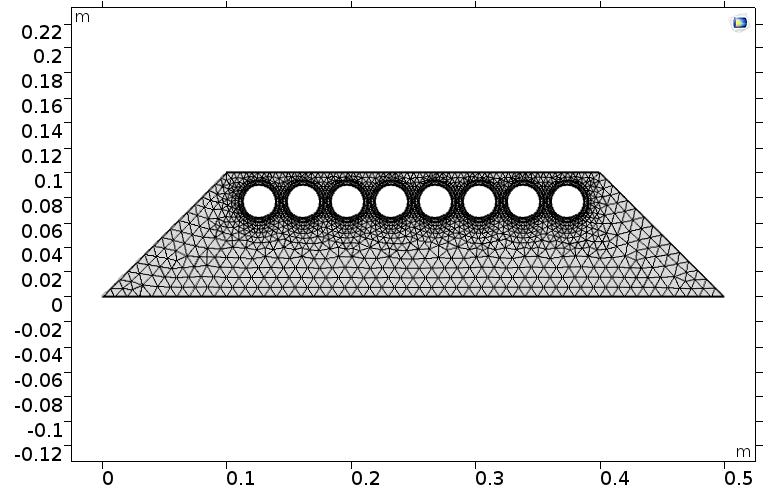
\includegraphics[width = 0.9\textwidth]{Mesh.png}
\caption{TCR Mesh}
\label{fig:TCRMesh}
\end{center}
\end{figure}

\begin{table}[H]
\centering
\caption{Grid independence test for TCR}
\label{tab:gridIndependenceTestMdelWithPipes}
\begin{tabular}{@{}|c|c|@{}}
\toprule
\textbf{Maximum Element Size (m)} & \textbf{Nusselt Number} \\ \midrule
0.0265                            & 41.790                  \\ \midrule
0.0185                            & 41.784                  \\ \midrule
0.01                              & 41.770                  \\ \midrule
0.005							&41.770						\\ \bottomrule
\end{tabular}
\end{table}

\subsection{Radiation resolution independence test}
Since this problem includes radiation model as well. Radiation resolution sensitivity has to be tested. For grid independence test in subsection \ref{subsec:gridIndTestPipeModel} radiation resolution was kept at maximum. Now, after fixing mesh element size radiation resolution is tested. Variation of Nusselt Number on the bottom glass is shown with varying radiation resolution in table \ref{tab:radResolutionIndTest}.

\begin{table}[H]
\centering
\caption{Radiation resolution independence test}
\label{tab:radResolutionIndTest}
\begin{tabular}{@{}|c|c|@{}}
\toprule
\textbf{Radiation Resolution} & \textbf{Nusselt Number} \\ \midrule
32                            & 41.675                  \\ \midrule
64                            & 41.760                  \\ \midrule
128                           & 41.764                  \\ \midrule
256                           & 41.770                  \\ \midrule
512                           & 41.771                  \\ \bottomrule
\end{tabular}
\end{table}

Finally, radiation resolution of 256 was selected as a further increment in radiation resolution does not improve accuracy significantly.

\subsection{Results}
Inside a trapezoidal cavity receiver the incoming heat energy from the reflectors is absorbed by the pipes and the cavity walls. A good fraction of this incoming heat energy is transferred to the working fluid flowing inside the pipes and rest of the fraction is lost to the environment via convection and radiation from the glass surface. The amount of energy which is lost to the environment is referred as total heat loss in this section. Efficiency for trapezoidal cavity receiver is defined as the fraction of incoming heat energy which is successfully transferred to the working fluid.

Heat loss analysis inside a trapezoidal cavity receiver has been performed for different mass flow rates of the working fluid using two different values of DNI over a day which includes 5 different timings- 08:00, 10:00, 12:00, 14:00 and 16:00 hrs. Total heat loss from the trapezoidal cavity receiver for DNI of 700 W/m\textsuperscript{2} and 800 W/m\textsuperscript{2} can be seen in the figures \ref{fig:TotalHeatLossDNI700} and \ref{fig:TotalHeatLossDNI800} respectively. 

\begin{figure}[H]
\begin{center}
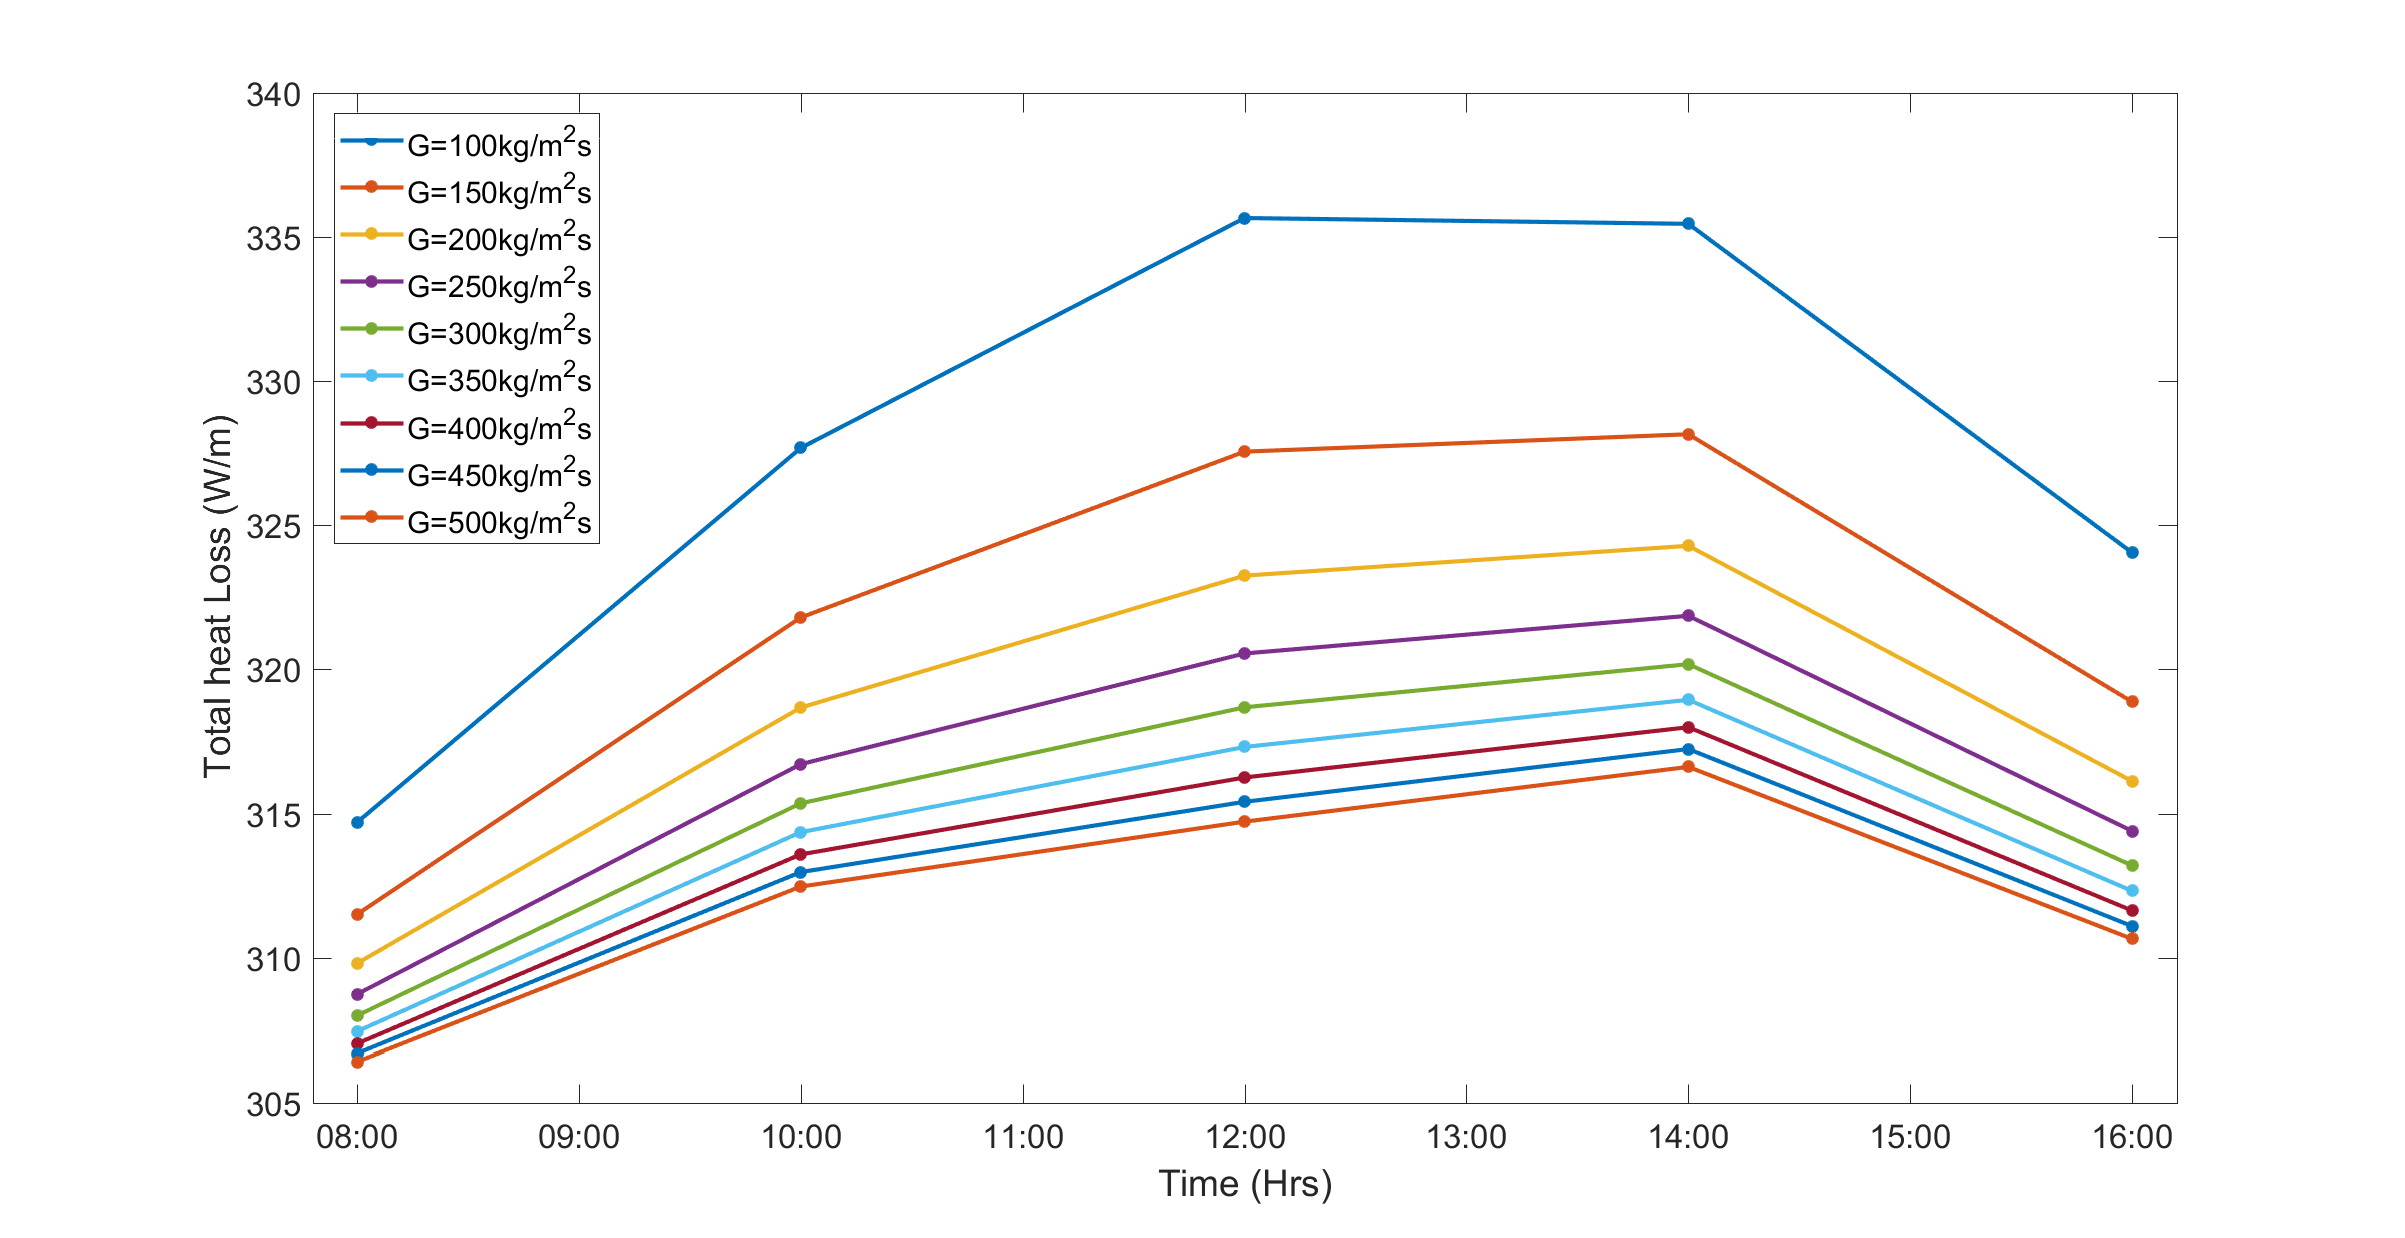
\includegraphics[width = \textwidth]{DNI700TotalHeatLossvariationwithmassflowrate.png}
\caption{Total heat loss from TCR: DNI 700 W/m\textsuperscript{2}}
\label{fig:TotalHeatLossDNI700}
\end{center}
\end{figure}


\begin{figure}[H]
\begin{center}
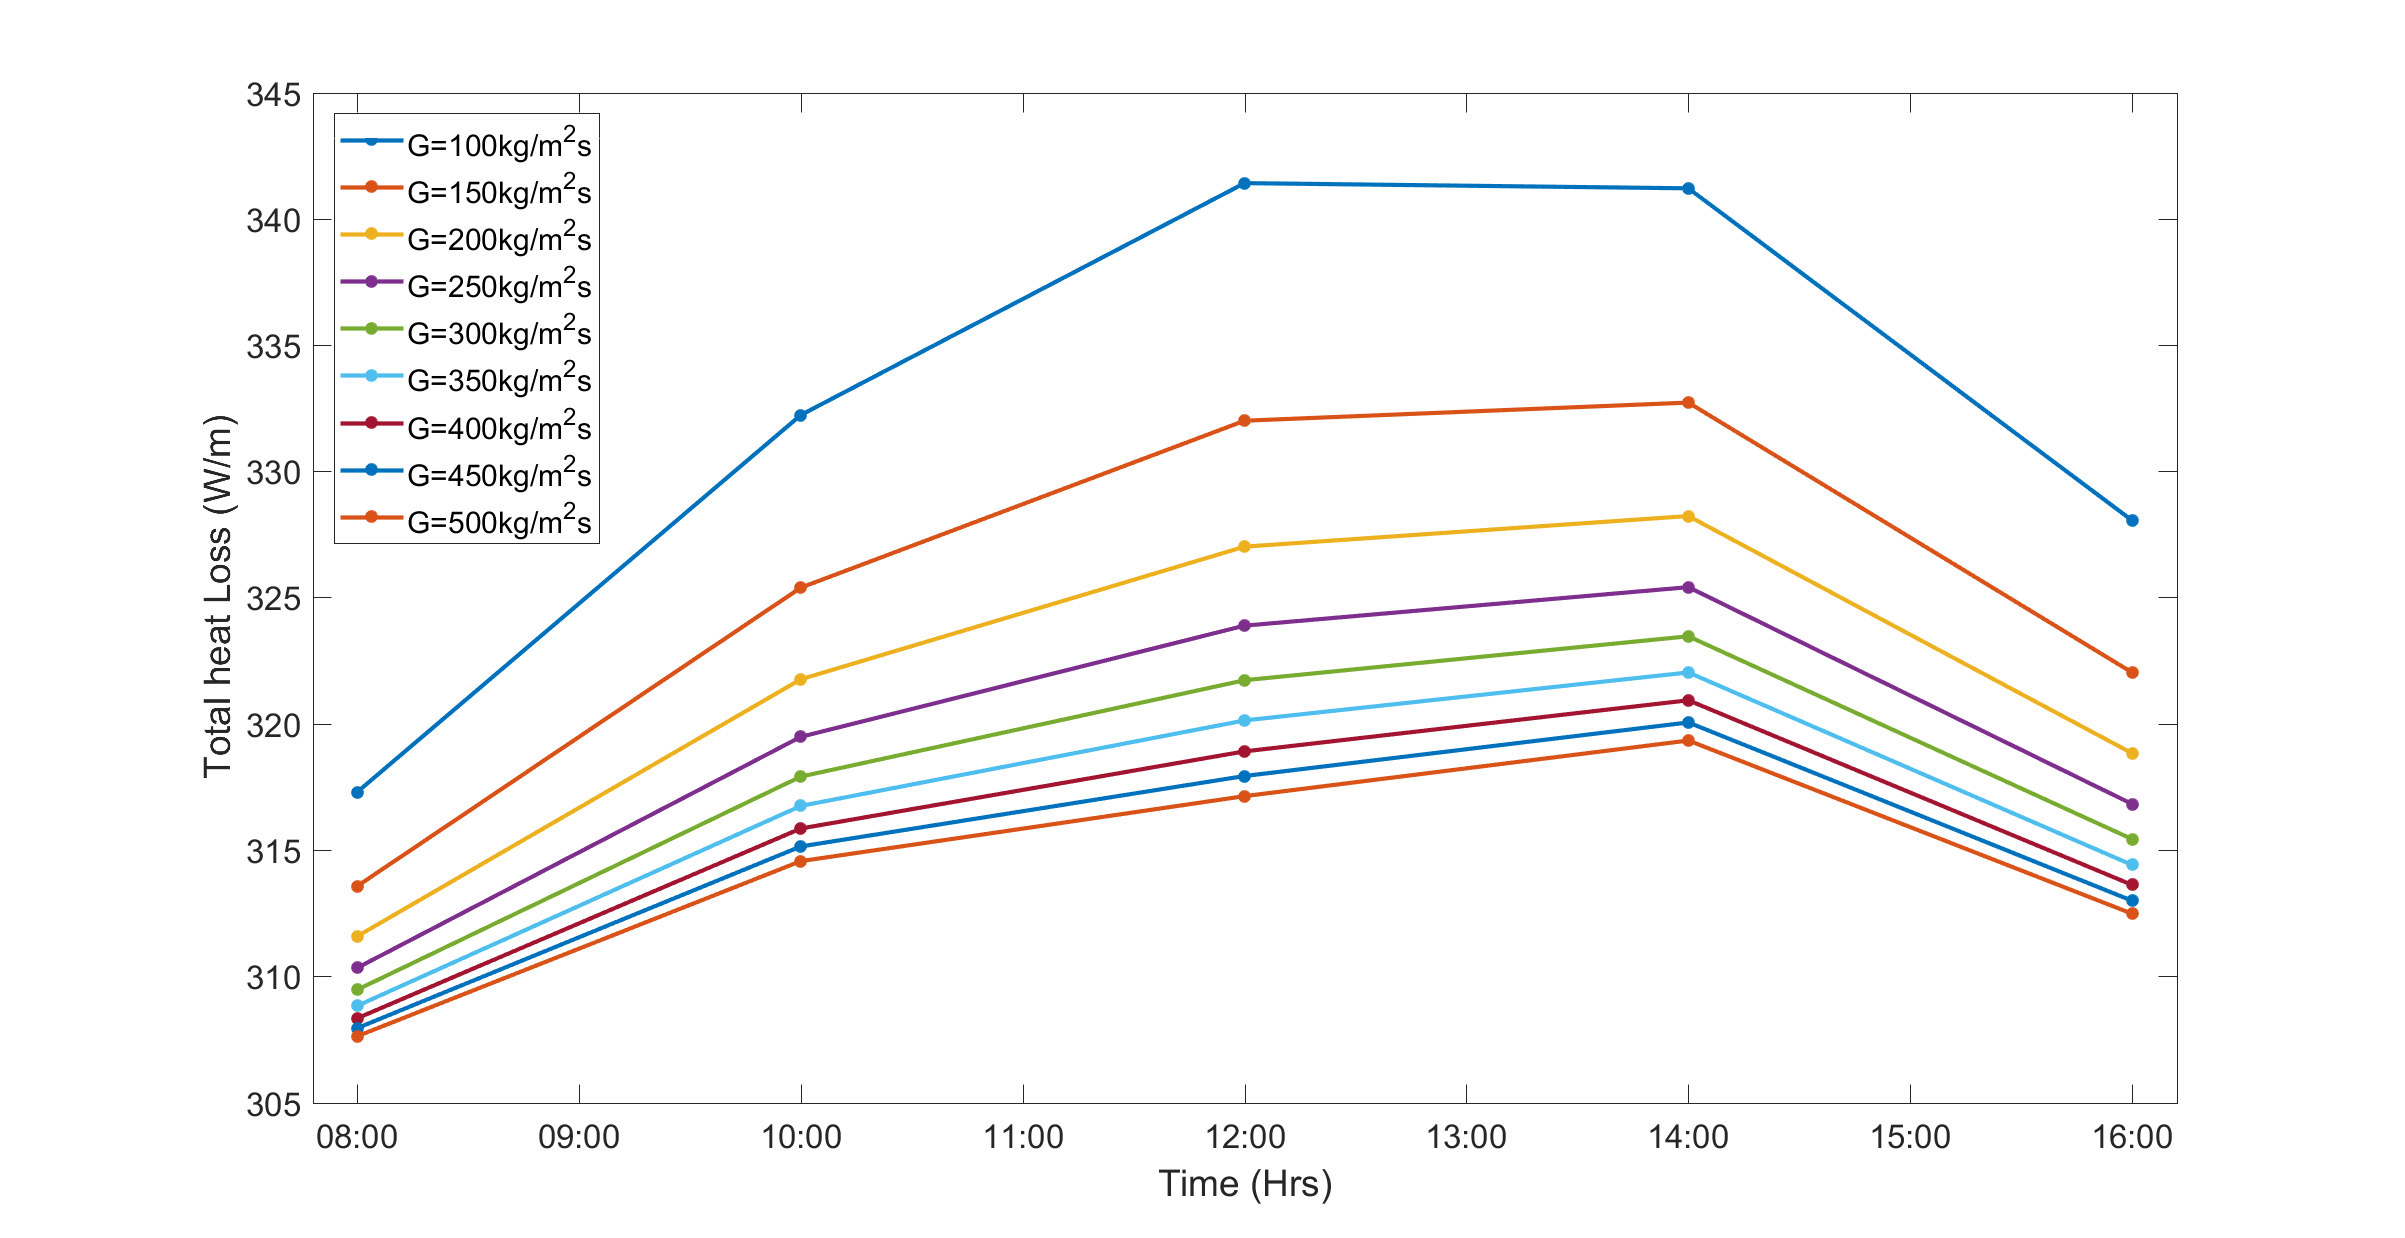
\includegraphics[width = \textwidth]{DNI800TotalHeatLossvariationwithmassflowrate.png}
\caption{Total heat loss from TCR: DNI 800 W/m\textsuperscript{2}}
\label{fig:TotalHeatLossDNI800}
\end{center}
\end{figure}


As the flow rate of the working fluid inside the pipes is increasing total heat loss from the cavity is decreasing. Because, heat is transferred from the pipes to working fluid through forced convection. Heat transfer coefficient for forced convection increases with increase in the mass flow rate. 

\begin{figure}[H]
\begin{center}
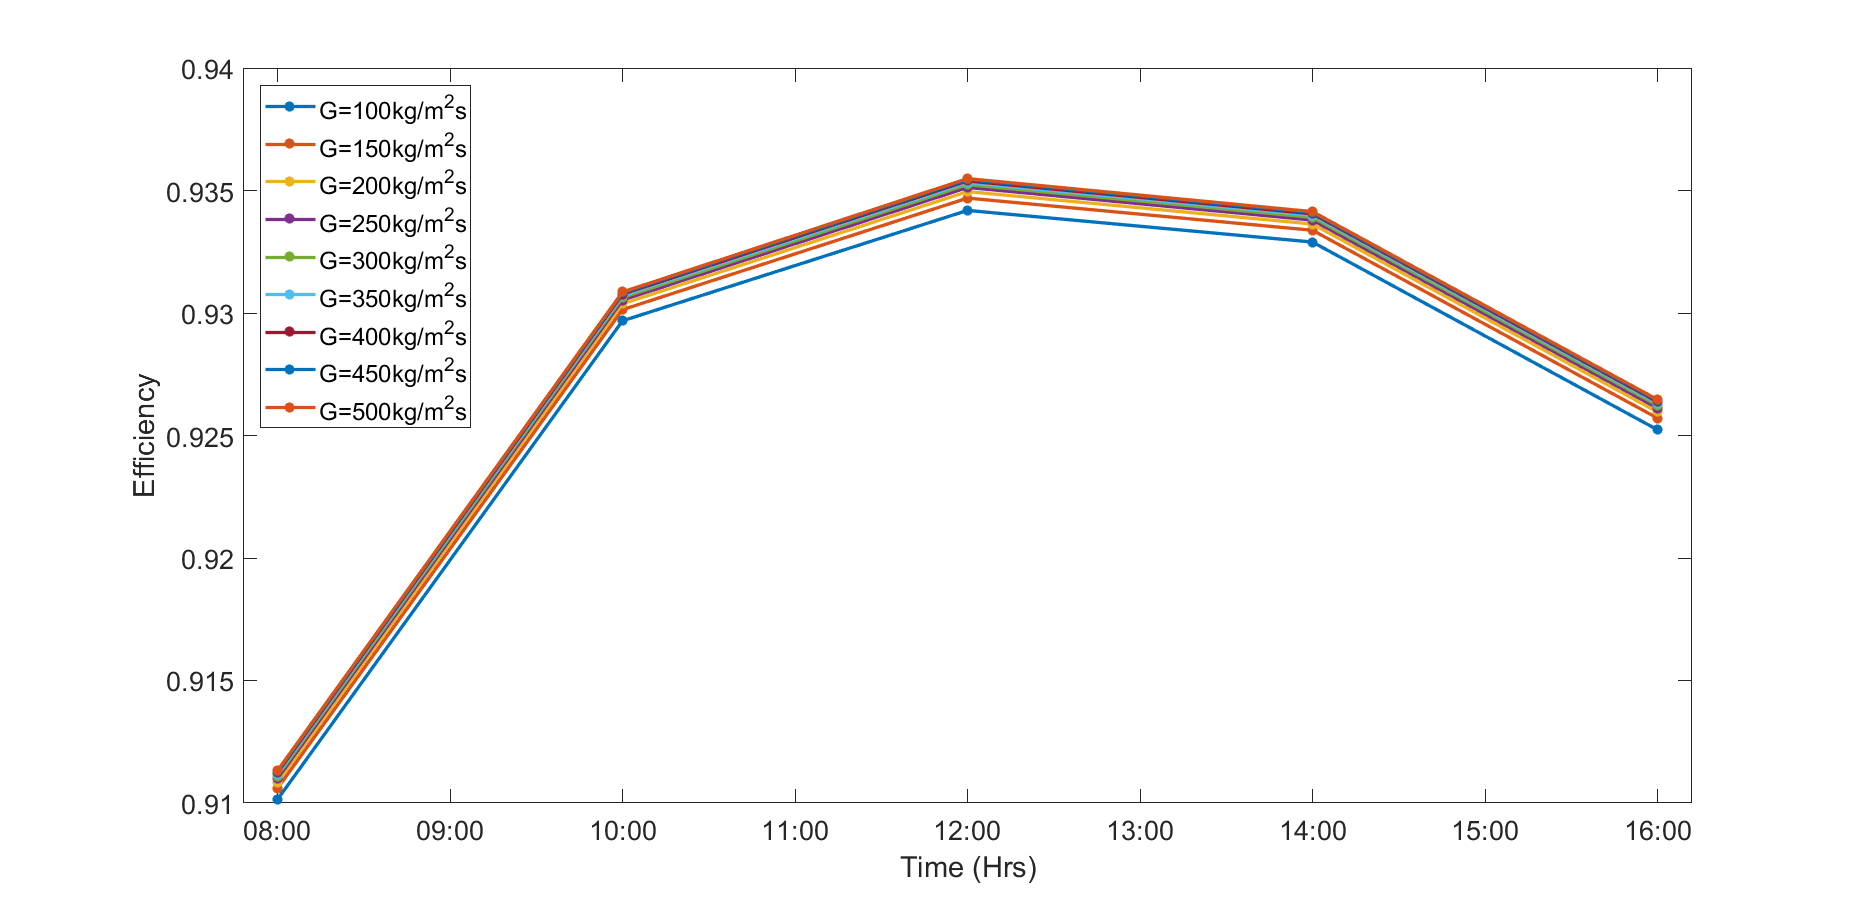
\includegraphics[width = \textwidth]{DNI700Efficiencyvariationwithmassflowrate.png}
\caption{TCR efficiency: DNI 700 W/m\textsuperscript{2}}
\label{fig:EffDNI700}
\end{center}
\end{figure}


\begin{figure}[H]
\begin{center}
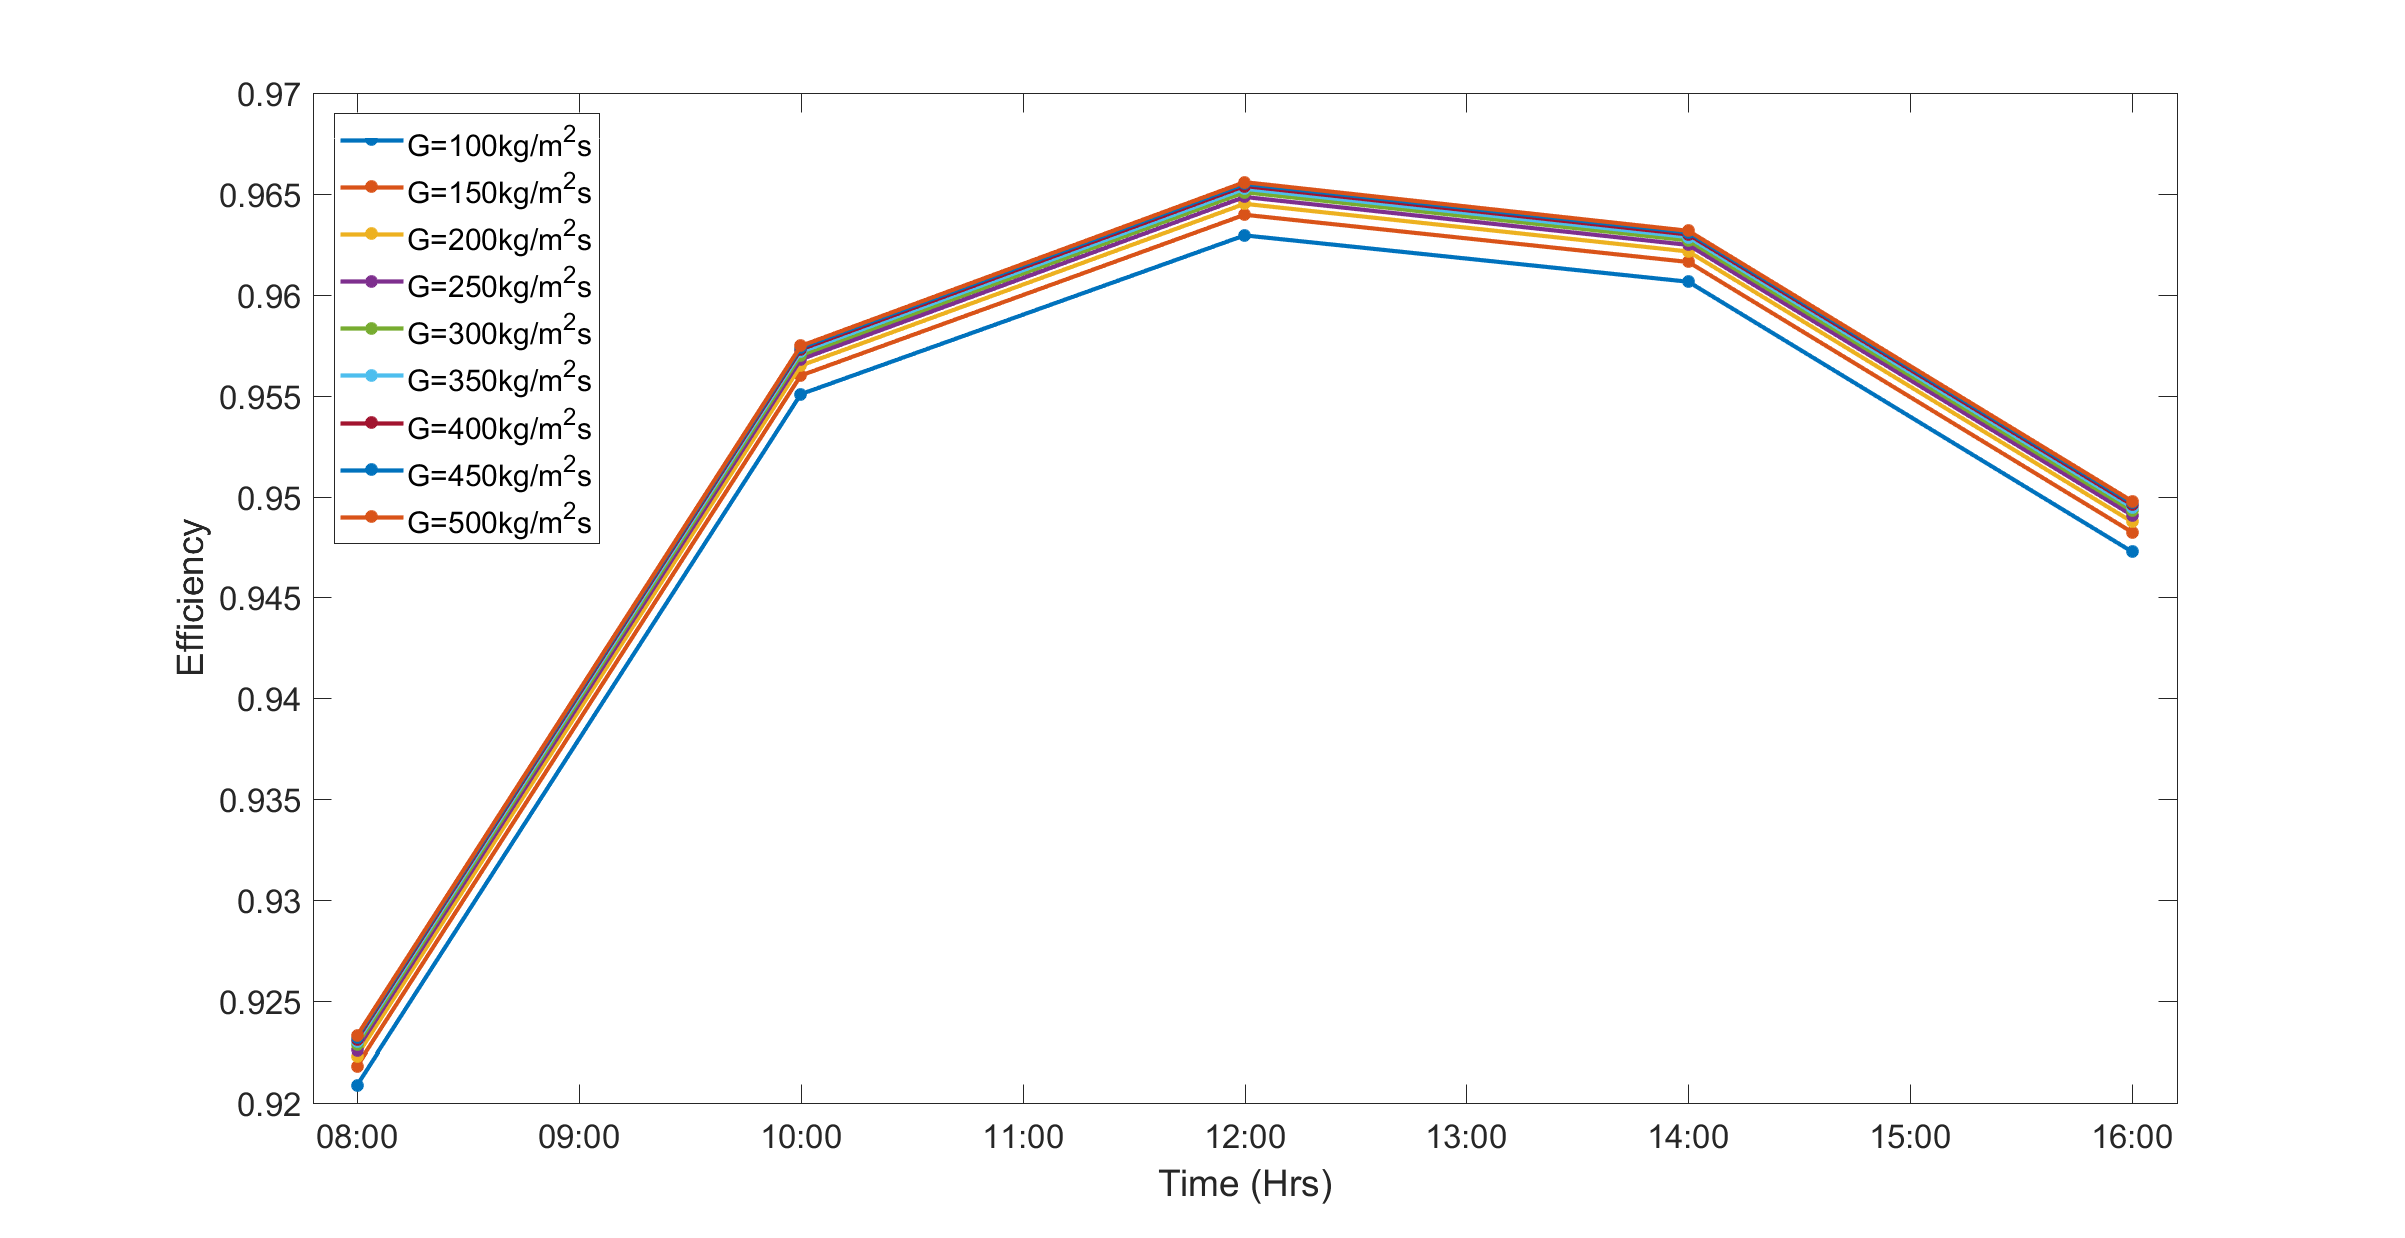
\includegraphics[width = \textwidth]{DNI800Efficiencyvariationwithmassflowrate.png}
\caption{TCR efficiency: DNI 800 W/m\textsuperscript{2}}
\label{fig:EffDNI800}
\end{center}
\end{figure}

Due to increase in the heat transfer coefficient, fraction of heat energy being transferred to the working fluid or efficiency increases and total heat loss decreases. Variation of efficiency over the for different mass flow rate can be sen in the figures \ref{fig:EffDNI700} and \ref{fig:EffDNI800}.

\begin{figure}[H]
\begin{center}
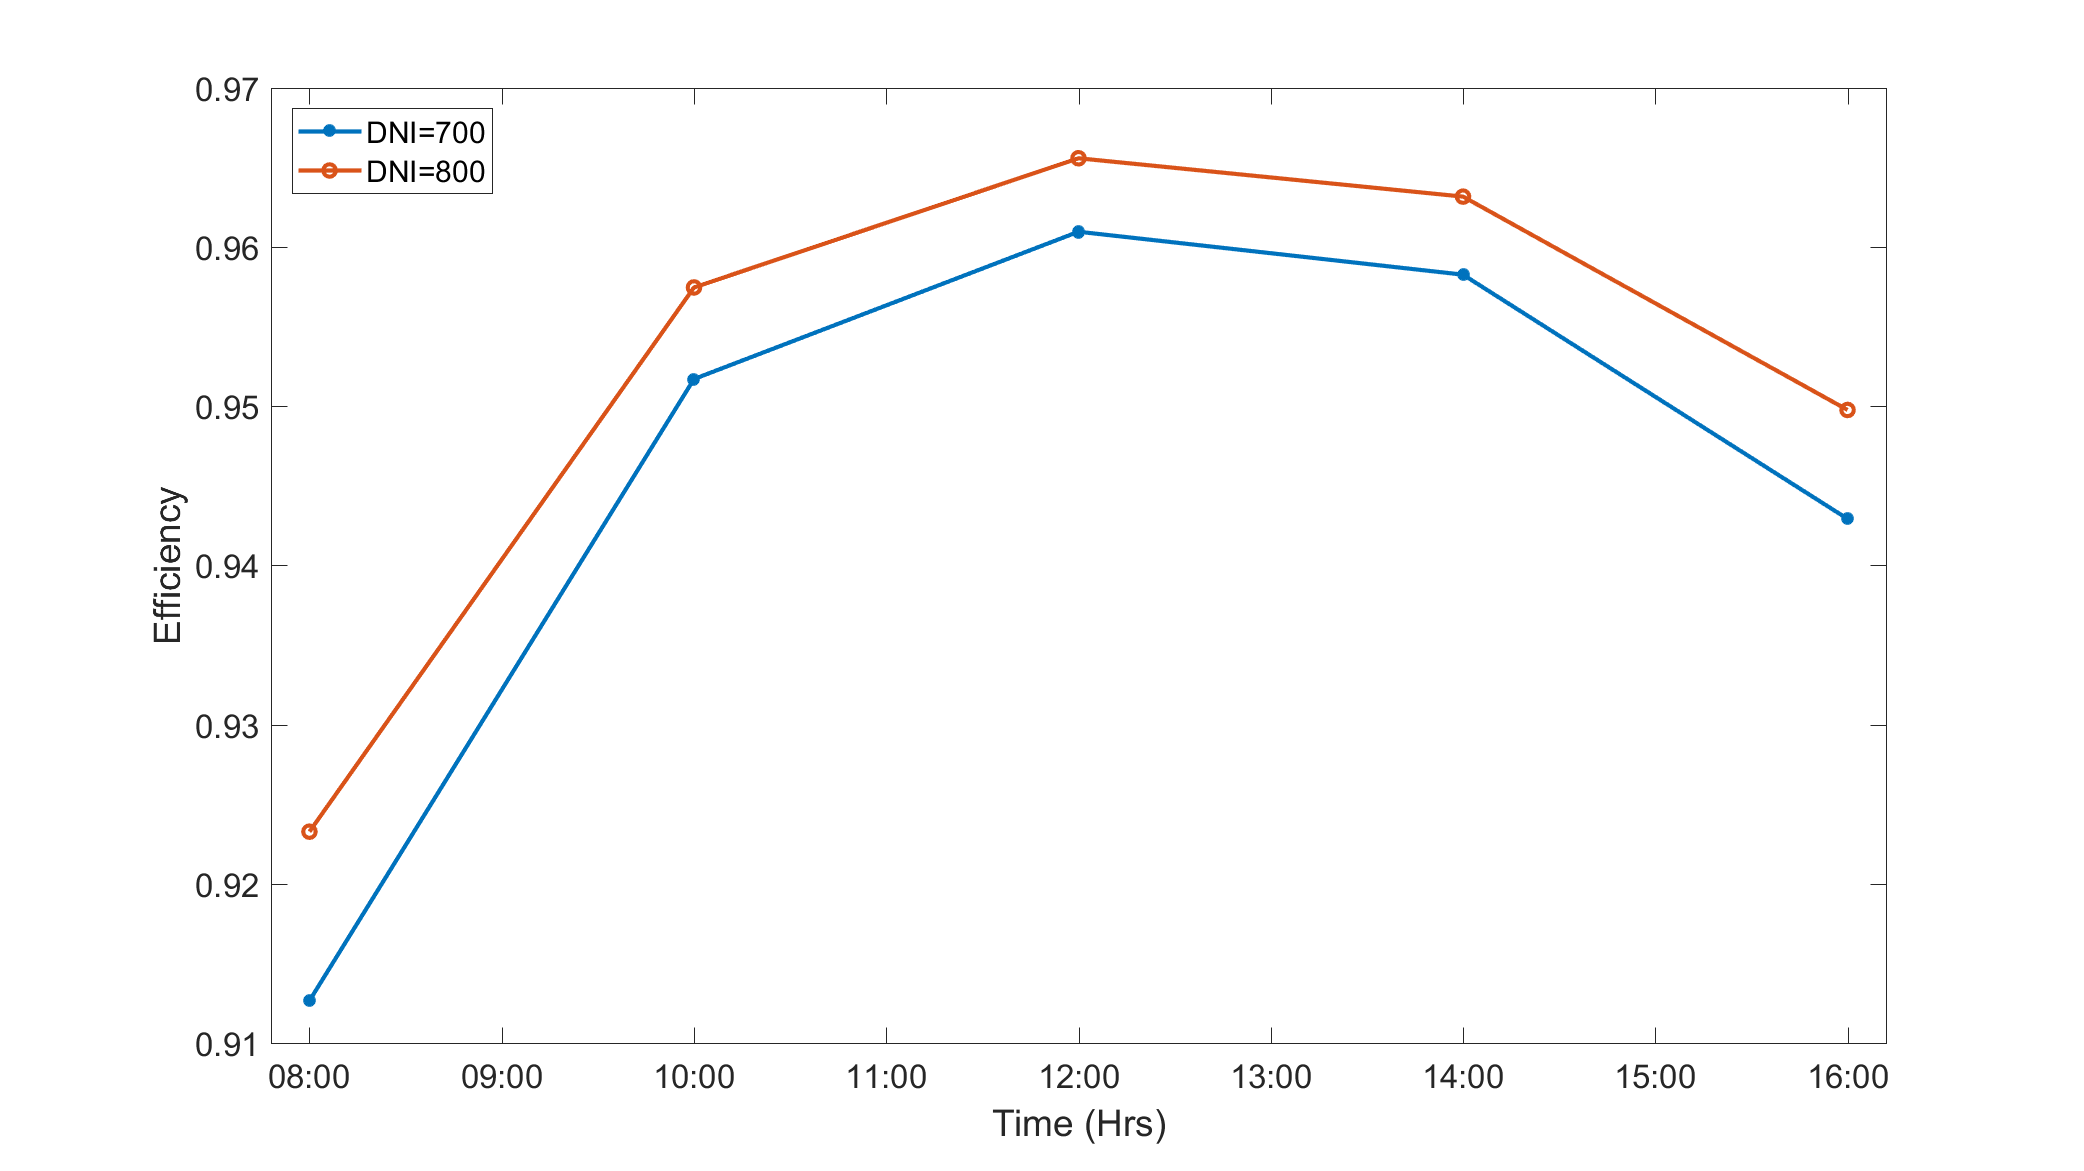
\includegraphics[width = \textwidth]{Efficiencyatmdot500forvaryingNDI.png}
\caption{TCR efficiency at G = 500 kg/m\textsuperscript{2}s}
\label{fig:EffG500}
\end{center}
\end{figure}
At a fixed mass flow rate of the working fluid, efficiency increases with increase in DNI. As DNI increases, total heat going inside the trapezoidal cavity receiver increases. Due to which pipes achieve higher temperature which can be seen in the fig. . Since convective heat transfer is directly proportional to temperature difference of the pipe and working fluid, increase in pipe temperature enhances the convection. Which in turn result into higher efficiency of the system which can be observed in the fig. \ref{fig:AvgTubeT}.

\begin{figure}[H]
\begin{center}
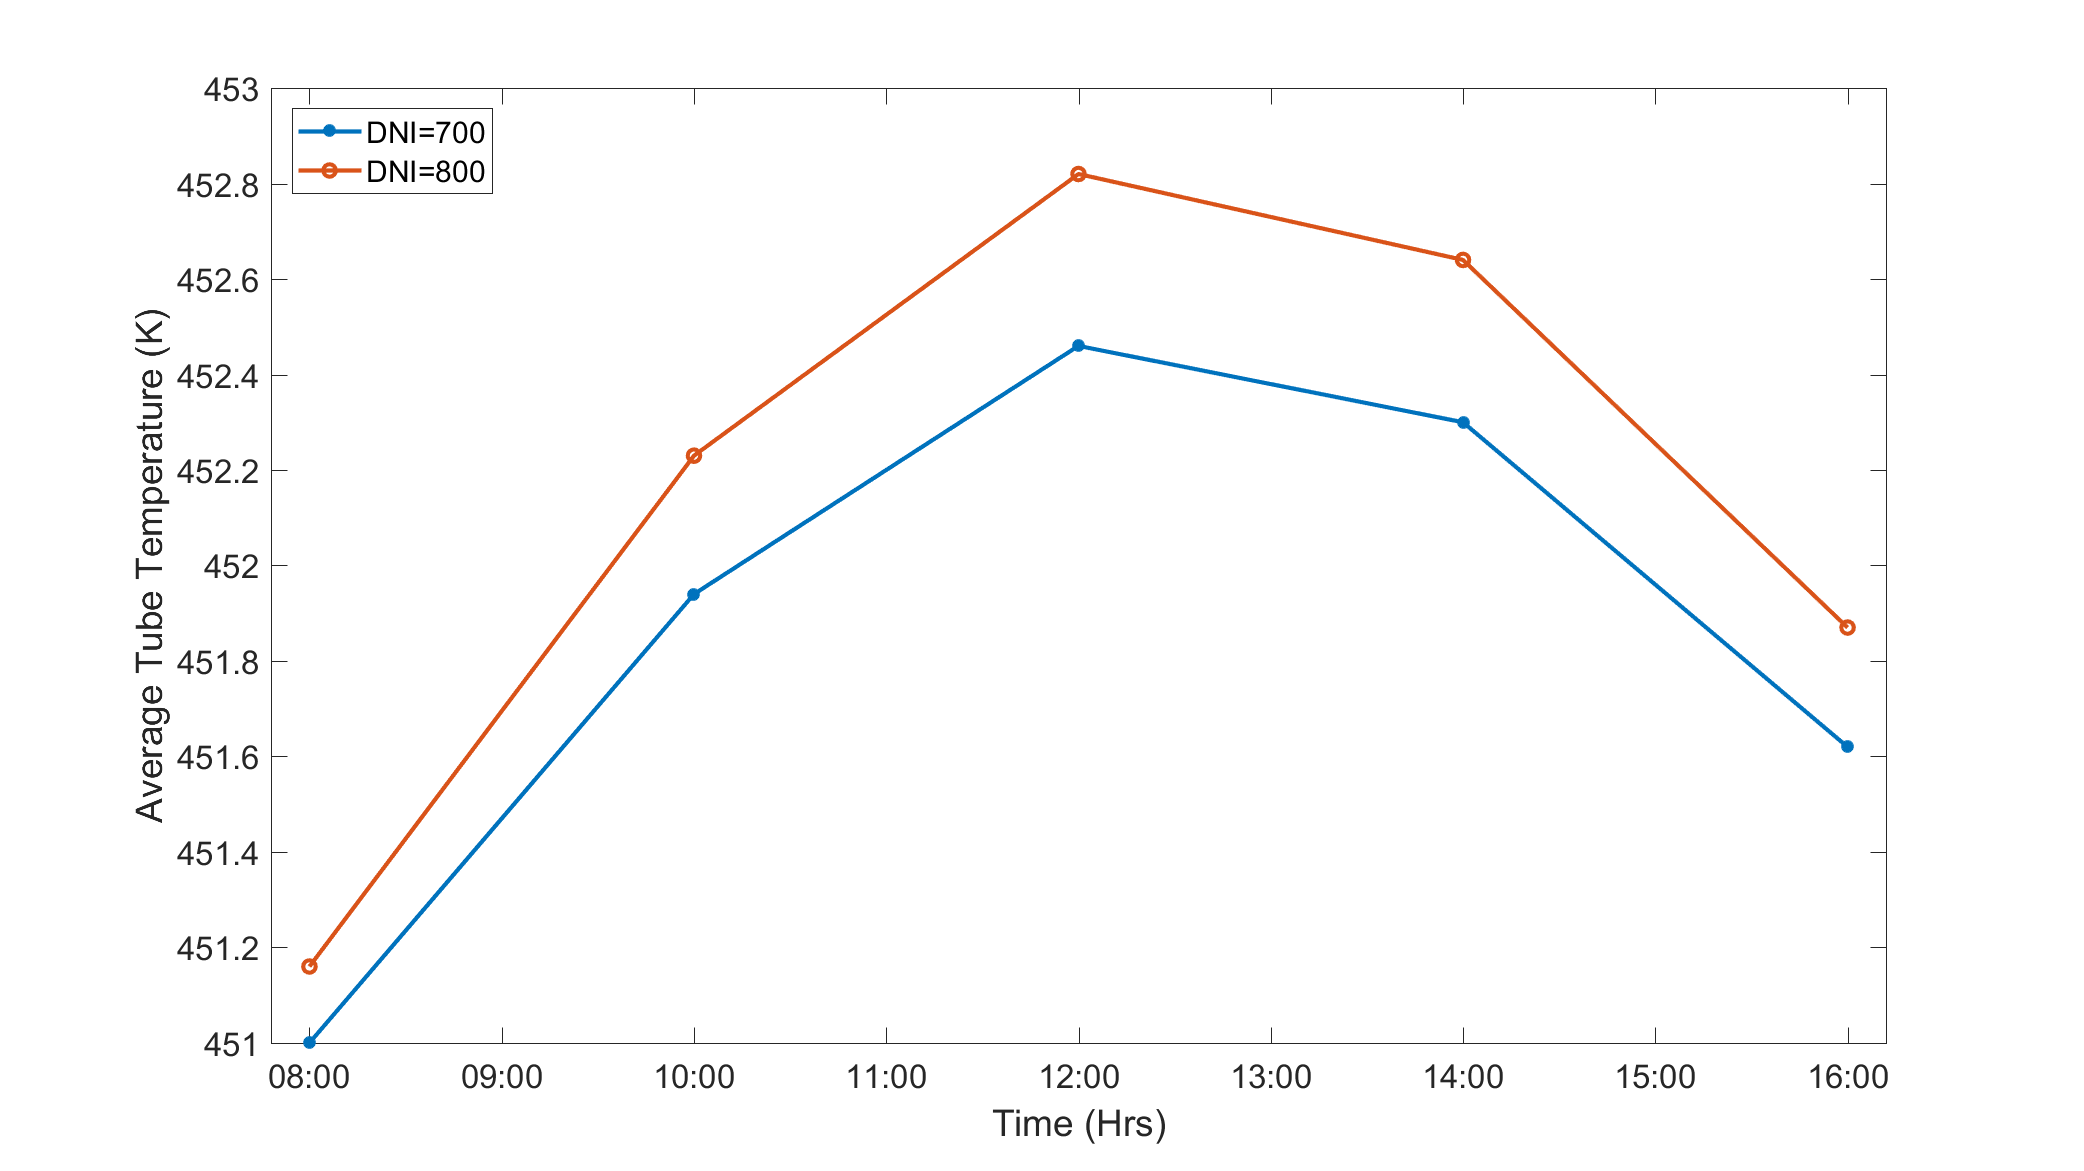
\includegraphics[width = \textwidth]{AvgTubeTatmdot500forvaryingNDI.png}
\caption{Average tube temperature at G = 500 kg/m\textsuperscript{2}s}
\label{fig:AvgTubeT}
\end{center}
\end{figure}

Heat loss coefficient has been calculated for different mass flow rate of the working fluid and for different DNI. Firstly Nussetl number has been calculated and then using Nusselt number heat loss coefficient has been obtained. Nusselt number is calculated using equation \ref{eq:Nu}
\begin{equation}\label{eq:Nu}
Nu_{l} = \frac{q"D}{K_{air}\Delta T}
\end{equation}
Let's consider physical model of trapezoidal cavity receiver. Useful heat is transferred to the working fluid which depends on the temperature of the pipe while heat loss is taking place at the glass surface which depends on the ambient air temperature. Here, goal is to calculate heat loss coefficient and two of the most important parameters which it depends upon are pipe temperature and ambient temperature. Keeping that in mind, $\delta \text{T}$ in the equation \ref{eq:Nu} has been taken to be the difference between pipe temperature and the ambient temperature. After calculation of Nusselt number, heat loss coefficient has been calculated using equation \ref{eq:U}. Its variation with mass flow rate of the working fluid can be seen in the fig. \ref{fig:UvariationwithG}.

\begin{equation}\label{eq:U}
U = Nu\frac{K_{air}}{D}
\end{equation}



\begin{figure}[H]
\begin{center}
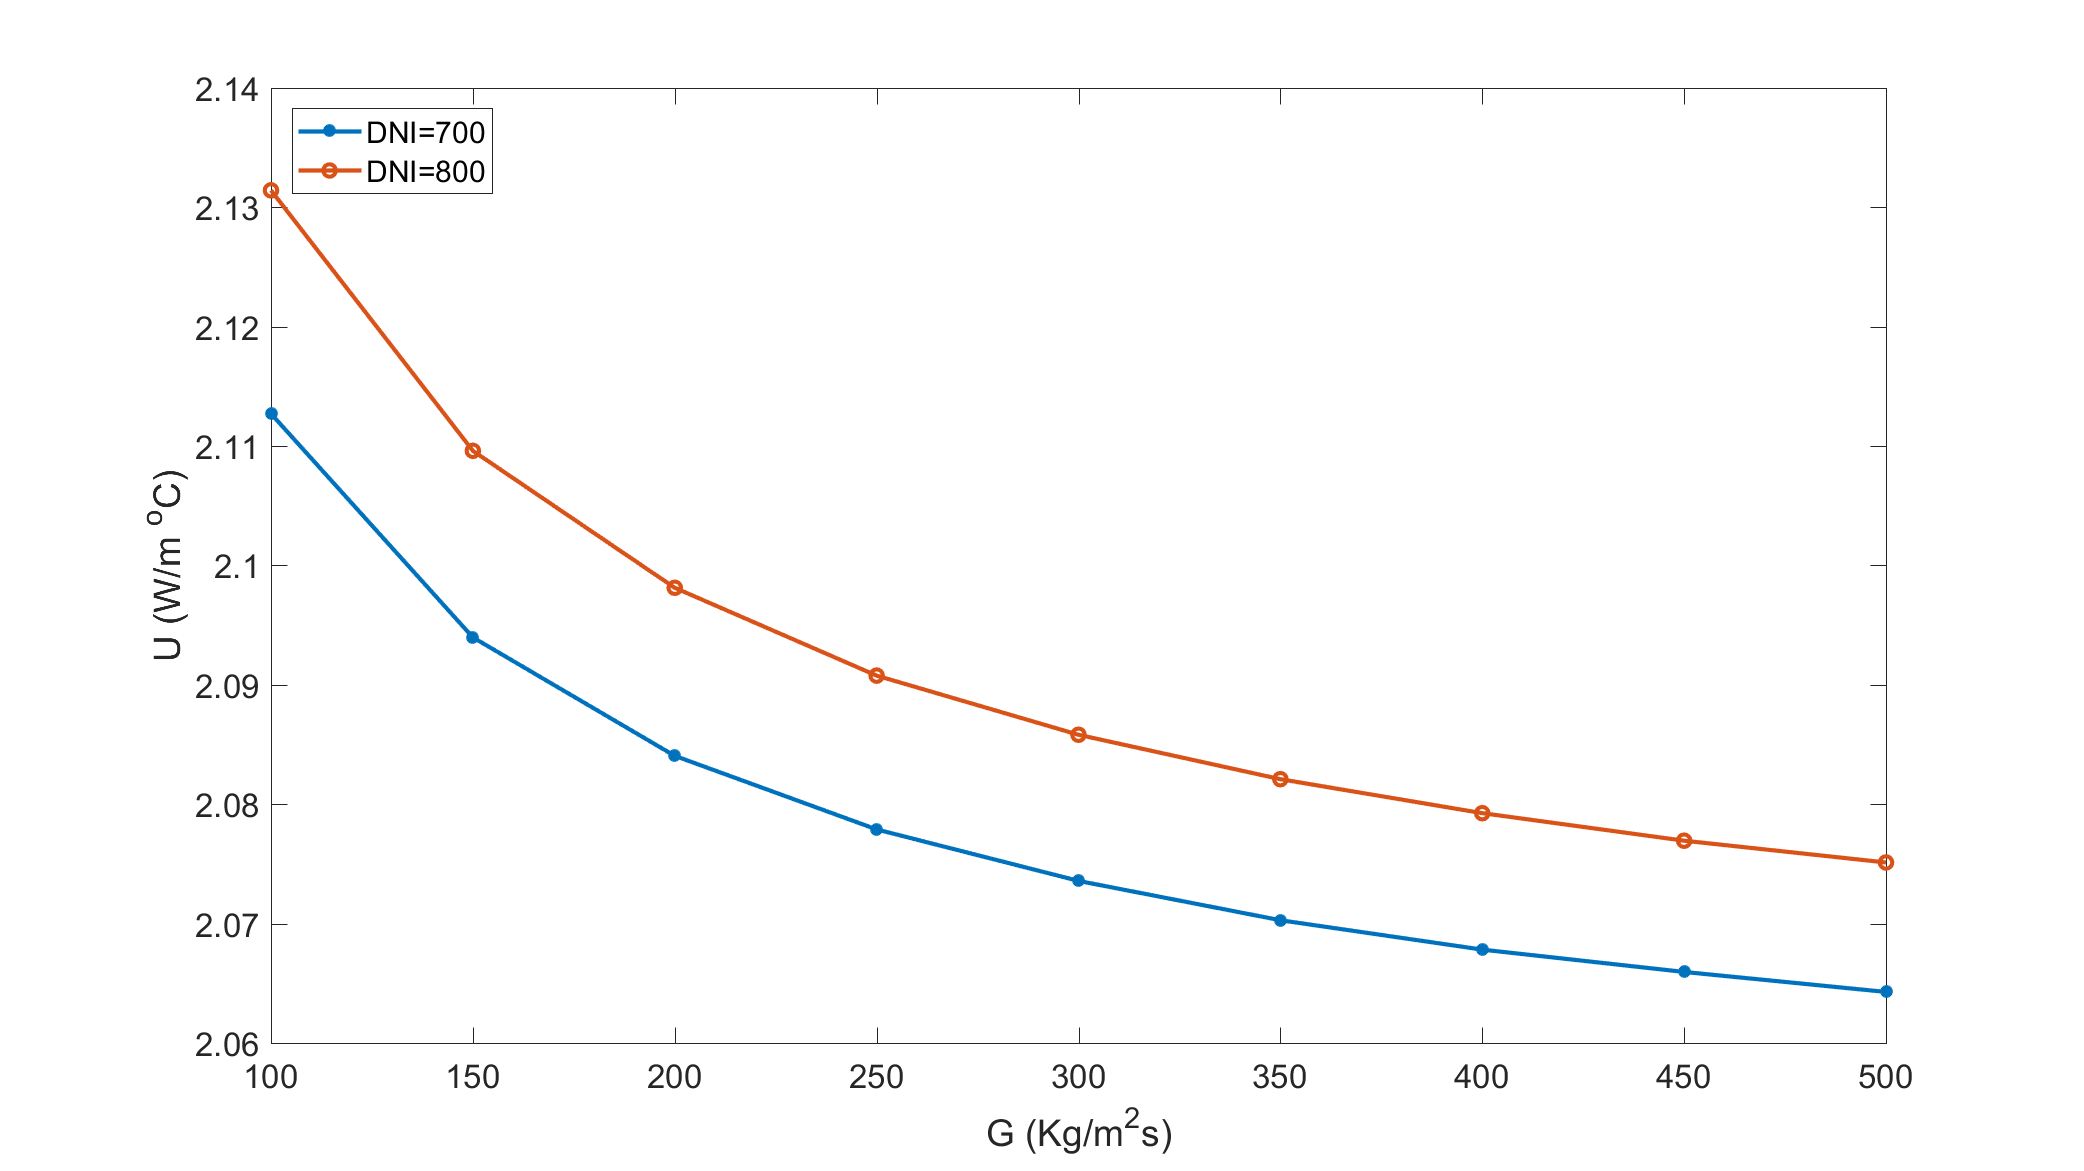
\includegraphics[width = \textwidth]{HeatLossCoeffatmdot500forvaryingNDI.png}
\caption{Variation of heat loss coefficient with mass flow rate at 1200 hrs}
\label{fig:UvariationwithG}
\end{center}
\end{figure}

\begin{figure}[H]
\begin{center}
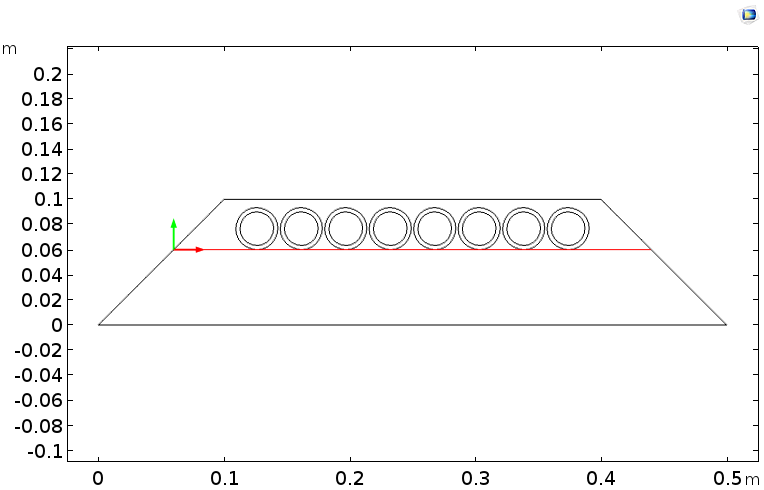
\includegraphics[width = \textwidth]{Cutline.png}
\caption{Cut Line: Tangent to the pipes}
\label{fig:cutline}
\end{center}
\end{figure}
To analyze temperature variation in the lateral direction a cut line has been defined just below the pipes such as it is a tangent to all the pipes which is shown in the fig. \ref{fig:cutline}. Temperature variation across this cut line has been shown in the fig. \ref{fig:Tcutline}.

\begin{figure}[H]
\begin{center}
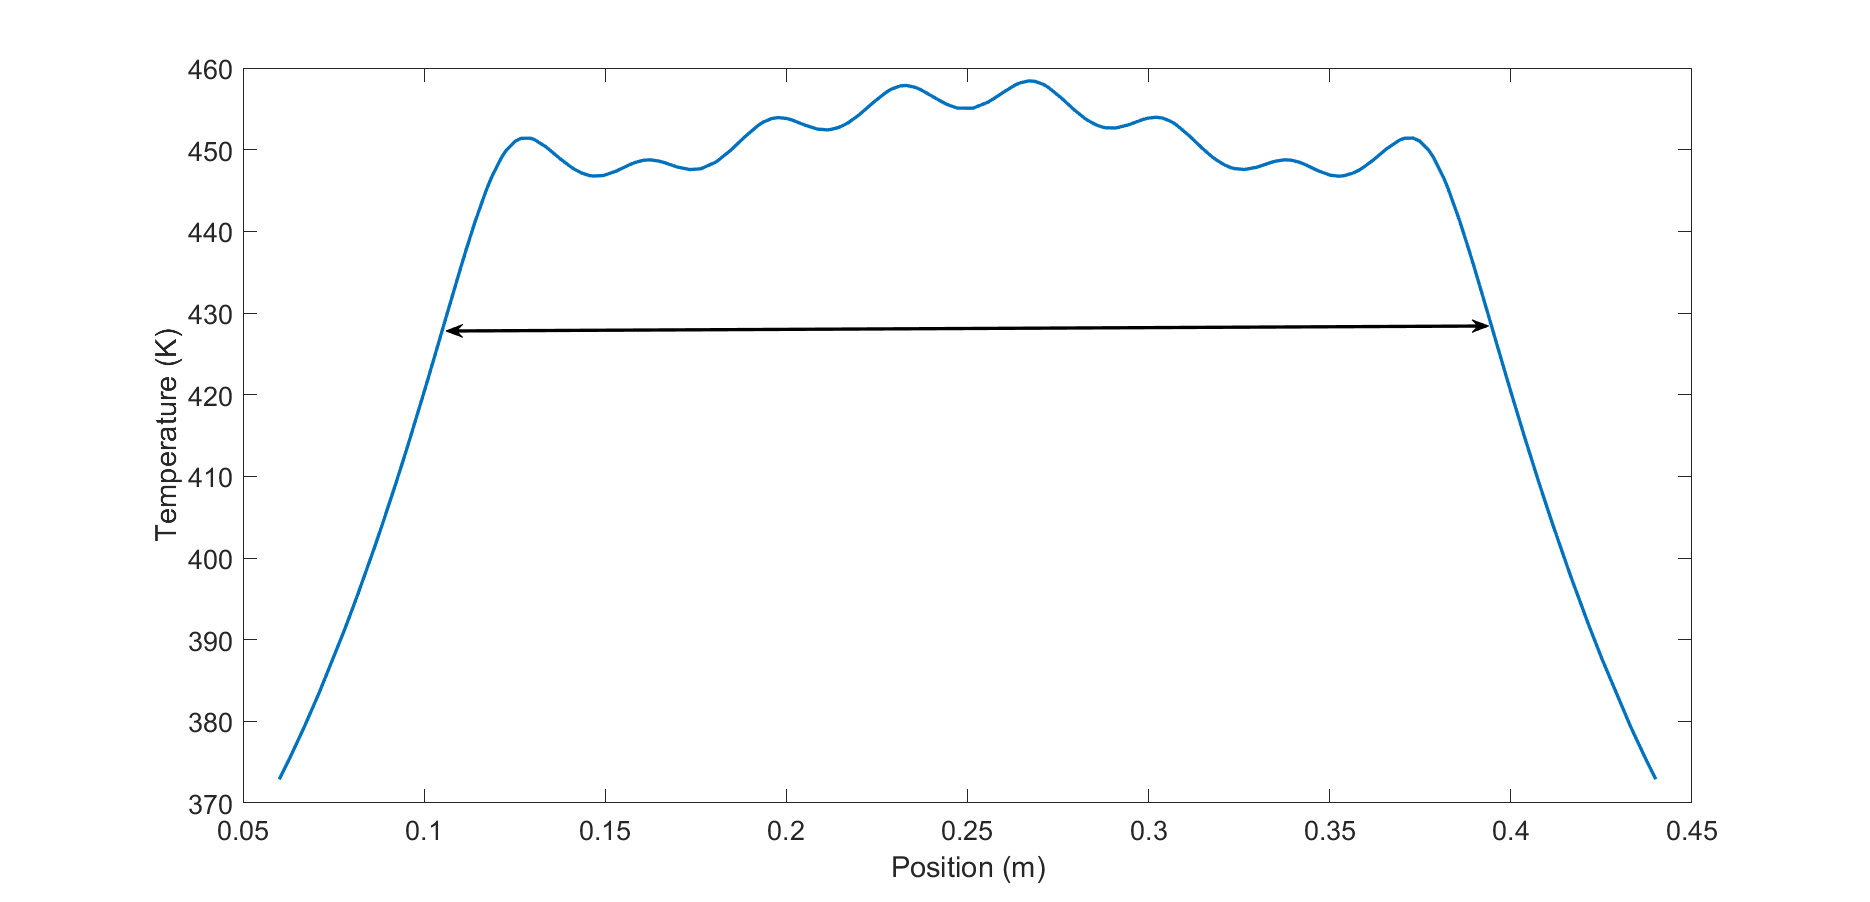
\includegraphics[width = \textwidth]{Tcutline_arrow.png}
\caption{Cut Line: Temperature variation for G = 100 kg/m\textsuperscript{2}s at 1200 hrs, DNI = 800 W/m\textsuperscript{2}}
\label{fig:Tcutline}
\end{center}
\end{figure}

Arrow in the fig. \ref{fig:Tcutline} show the spread of the tubes. Temperature in this plot provides understanding of temperature variation of nearby air. Within the spread of pipes, maximum temperature difference of 30 \textsuperscript{0}C can be seen over the length of approximately 0.15 m in the lateral direction. Thus temperature gradient in the lateral direction is roughly 200 K/m. Now, consider the vertical direction. Average temperature of the top wall is 465.1 K and the same for bottom glass is 340.6 K. Depth of the cavity is 0.1 m which results into vertical temperature gradient of 1245 K/m. Vertical temperature gradient is more than 6 times than the lateral temperature gradient. And this is maximum lateral temperature gradient that can exist for the given study as this calculation is being done for the least mass flow rate of the working fluid and at 12:00 hrs. As the mass flow rate increases vertical temperature gradient decreases. So even in the worst case scenario, Vertical temperature gradient very large than the lateral temperature gradient. As explained in the beginning of the chapter \ref{ch_Heat_Transfer}, lateral temperature gradient is responsible for convective currents while vertical temperature gradient has nothing to do with it. And though the lateral temperature gradient exists but most of heat transfer is done by conduction only as by Mohan et. al.\citep{MOHAN201837}. No doubt, some small convective currents will form but its contribution in the overall heat transfer can be  neglected. on more thing to notice is that the temperature gradient would be more than 200 \textsuperscript{0}C if length beyond the spread of the pipes is considered but, that extra length is very small which will avert formation of any significant convection current despite of temperature gradient. This is the case just below the pipes. As we go down lateral temperature gradient fades out which can be seen in the isothermal contour \ref{fig:isothermG1001200hrs}. Flat isotherms suggest absence of convection. Even though lateral temperature gradient exists, it does so within very small thickness just below the pipes which supports our assumption of negligible convection.

\begin{figure}[H]
\begin{center}
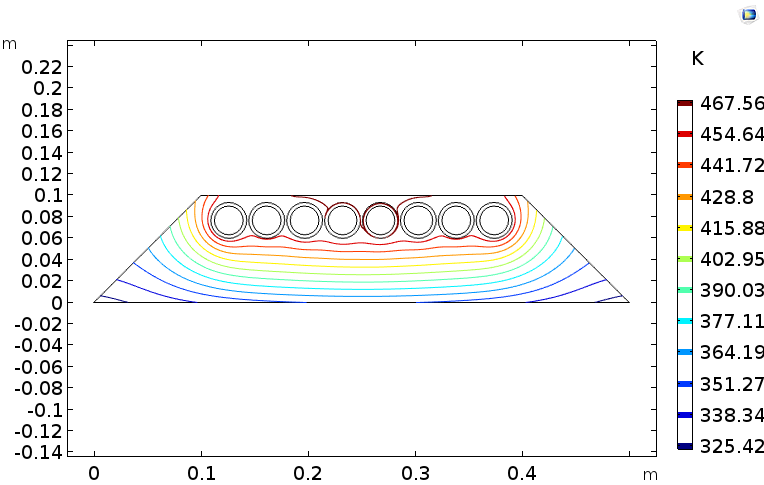
\includegraphics[width = \textwidth]{isothermalContour.png}
\caption{Isothermal contour for G = 100 kg/m\textsuperscript{2}s at 1200 hrs, DNI = 800 W/m\textsuperscript{2}}
\label{fig:isothermG1001200hrs}
\end{center}
\end{figure} 



Temperature variation of the pipes has been observed with the variation of mass flow rate of the working fluid. Since temperature is symmetrical, temperature of only 4 tubes are shown in the table \ref{tab:pipeT}. For nomenclature of the pipes please refer to fig.
Let's consider the first row which corresponds to mass flow rate of 100 kg/m\textsuperscript{2}s. Maximum difference of pipe temperature is roughly 9 \textsuperscript{o}C between temperature of pipe 1 and 3. While for last row which corresponds to mass flow rate of 500 kg/m\textsuperscript{2}s. Maximum difference of pipe temperature is roughly 2.5 \textsuperscript{o}C. It can be observed from the table that as the mass flow rate increases, all the pipes tend to converge to a uniform temperature. This is important as many researchers{give reference} have performed heat loss analysis by assuming that pipes are at uniform temperature. It turns out that at higher mass flow rates that assumption is right with a high degree of accuracy.


\begin{figure}[H]
\begin{center}
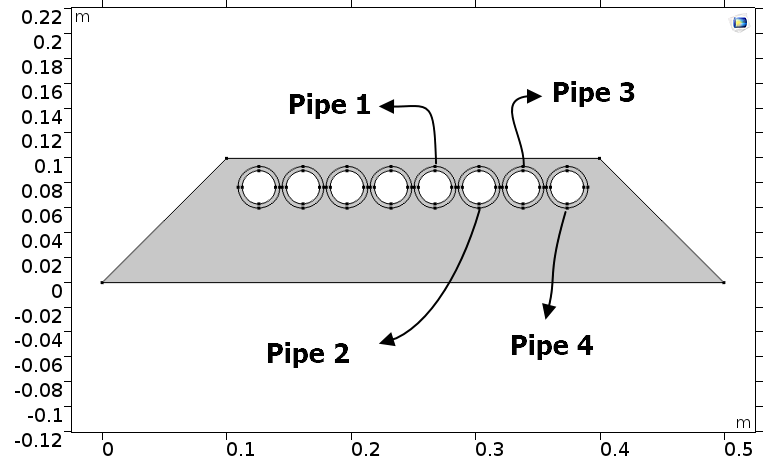
\includegraphics[width = \textwidth]{pipeNomenclatureEdit.png}
\caption{Isothermal contour for G = 100 kg/m\textsuperscript{2}s at 1200 hrs}
\label{fig:isothermG1001200hrs}
\end{center}
\end{figure} 

\begin{table}[H]
\centering
\caption{Pipe Temperature Variation with Mass Flow Rate at 1200 hrs, DNI = 800 W/m\textsuperscript{2}}
\label{tab:pipeT}
\begin{tabular}{@{}|c|c|c|c|c|@{}}
\toprule
\multirow{2}{*}{\textbf{\begin{tabular}[c]{@{}c@{}}Mass Flow Rate \\ (kg/m2s)\end{tabular}}} & \multicolumn{4}{c|}{\textbf{Temperature}}                             \\ \cmidrule(l){2-5} 
                                                                                             & \textbf{Pipe 1} & \textbf{Pipe 2} & \textbf{Pipe 3} & \textbf{Pipe 4} \\ \midrule
100                                                                                          & 464.38          & 460.34          & 455.67          & 460.67          \\ \midrule
200                                                                                          & 456.15          & 458.28          & 455.95          & 453.25          \\ \midrule
300                                                                                          & 455.99          & 454.30          & 452.35          & 454.45          \\ \midrule
400                                                                                          & 454.76          & 453.42          & 451.86          & 453.54          \\ \midrule
500                                                                                          & 453.98          & 452.86          & 451.56          & 452.96          \\ \bottomrule
\end{tabular}
\end{table}




